\documentclass[1p]{elsarticle_modified}
%\bibliographystyle{elsarticle-num}

%\usepackage[colorlinks]{hyperref}
%\usepackage{abbrmath_seonhwa} %\Abb, \Ascr, \Acal ,\Abf, \Afrak
\usepackage{amsfonts}
\usepackage{amssymb}
\usepackage{amsmath}
\usepackage{amsthm}
\usepackage{scalefnt}
\usepackage{amsbsy}
\usepackage{kotex}
\usepackage{caption}
\usepackage{subfig}
\usepackage{color}
\usepackage{graphicx}
\usepackage{xcolor} %% white, black, red, green, blue, cyan, magenta, yellow
\usepackage{float}
\usepackage{setspace}
\usepackage{hyperref}

\usepackage{tikz}
\usetikzlibrary{arrows}

\usepackage{multirow}
\usepackage{array} % fixed length table
\usepackage{hhline}

%%%%%%%%%%%%%%%%%%%%%
\makeatletter
\renewcommand*\env@matrix[1][\arraystretch]{%
	\edef\arraystretch{#1}%
	\hskip -\arraycolsep
	\let\@ifnextchar\new@ifnextchar
	\array{*\c@MaxMatrixCols c}}
\makeatother %https://tex.stackexchange.com/questions/14071/how-can-i-increase-the-line-spacing-in-a-matrix
%%%%%%%%%%%%%%%

\usepackage[normalem]{ulem}

\newcommand{\msout}[1]{\ifmmode\text{\sout{\ensuremath{#1}}}\else\sout{#1}\fi}
%SOURCE: \msout is \stkout macro in https://tex.stackexchange.com/questions/20609/strikeout-in-math-mode

\newcommand{\cancel}[1]{
	\ifmmode
	{\color{red}\msout{#1}}
	\else
	{\color{red}\sout{#1}}
	\fi
}

\newcommand{\add}[1]{
	{\color{blue}\uwave{#1}}
}

\newcommand{\replace}[2]{
	\ifmmode
	{\color{red}\msout{#1}}{\color{blue}\uwave{#2}}
	\else
	{\color{red}\sout{#1}}{\color{blue}\uwave{#2}}
	\fi
}

\newcommand{\Sol}{\mathcal{S}} %segment
\newcommand{\D}{D} %diagram
\newcommand{\A}{\mathcal{A}} %arc


%%%%%%%%%%%%%%%%%%%%%%%%%%%%%5 test

\def\sl{\operatorname{\textup{SL}}(2,\Cbb)}
\def\psl{\operatorname{\textup{PSL}}(2,\Cbb)}
\def\quan{\mkern 1mu \triangleright \mkern 1mu}

\theoremstyle{definition}
\newtheorem{thm}{Theorem}[section]
\newtheorem{prop}[thm]{Proposition}
\newtheorem{lem}[thm]{Lemma}
\newtheorem{ques}[thm]{Question}
\newtheorem{cor}[thm]{Corollary}
\newtheorem{defn}[thm]{Definition}
\newtheorem{exam}[thm]{Example}
\newtheorem{rmk}[thm]{Remark}
\newtheorem{alg}[thm]{Algorithm}

\newcommand{\I}{\sqrt{-1}}
\begin{document}

%\begin{frontmatter}
%
%\title{Boundary parabolic representations of knots up to 8 crossings}
%
%%% Group authors per affiliation:
%\author{Yunhi Cho} 
%\address{Department of Mathematics, University of Seoul, Seoul, Korea}
%\ead{yhcho@uos.ac.kr}
%
%
%\author{Seonhwa Kim} %\fnref{s_kim}}
%\address{Center for Geometry and Physics, Institute for Basic Science, Pohang, 37673, Korea}
%\ead{ryeona17@ibs.re.kr}
%
%\author{Hyuk Kim}
%\address{Department of Mathematical Sciences, Seoul National University, Seoul 08826, Korea}
%\ead{hyukkim@snu.ac.kr}
%
%\author{Seokbeom Yoon}
%\address{Department of Mathematical Sciences, Seoul National University, Seoul, 08826,  Korea}
%\ead{sbyoon15@snu.ac.kr}
%
%\begin{abstract}
%We find all boundary parabolic representation of knots up to 8 crossings.
%
%\end{abstract}
%\begin{keyword}
%    \MSC[2010] 57M25 
%\end{keyword}
%
%\end{frontmatter}

%\linenumbers
%\tableofcontents
%
\newcommand\colored[1]{\textcolor{white}{\rule[-0.35ex]{0.8em}{1.4ex}}\kern-0.8em\color{red} #1}%
%\newcommand\colored[1]{\textcolor{white}{ #1}\kern-2.17ex	\textcolor{white}{ #1}\kern-1.81ex	\textcolor{white}{ #1}\kern-2.15ex\color{red}#1	}

{\Large $\underline{12a_{0242}~(K12a_{0242})}$}

\setlength{\tabcolsep}{10pt}
\renewcommand{\arraystretch}{1.6}
\vspace{1cm}\begin{tabular}{m{100pt}>{\centering\arraybackslash}m{274pt}}
\multirow{5}{120pt}{
	\centering
	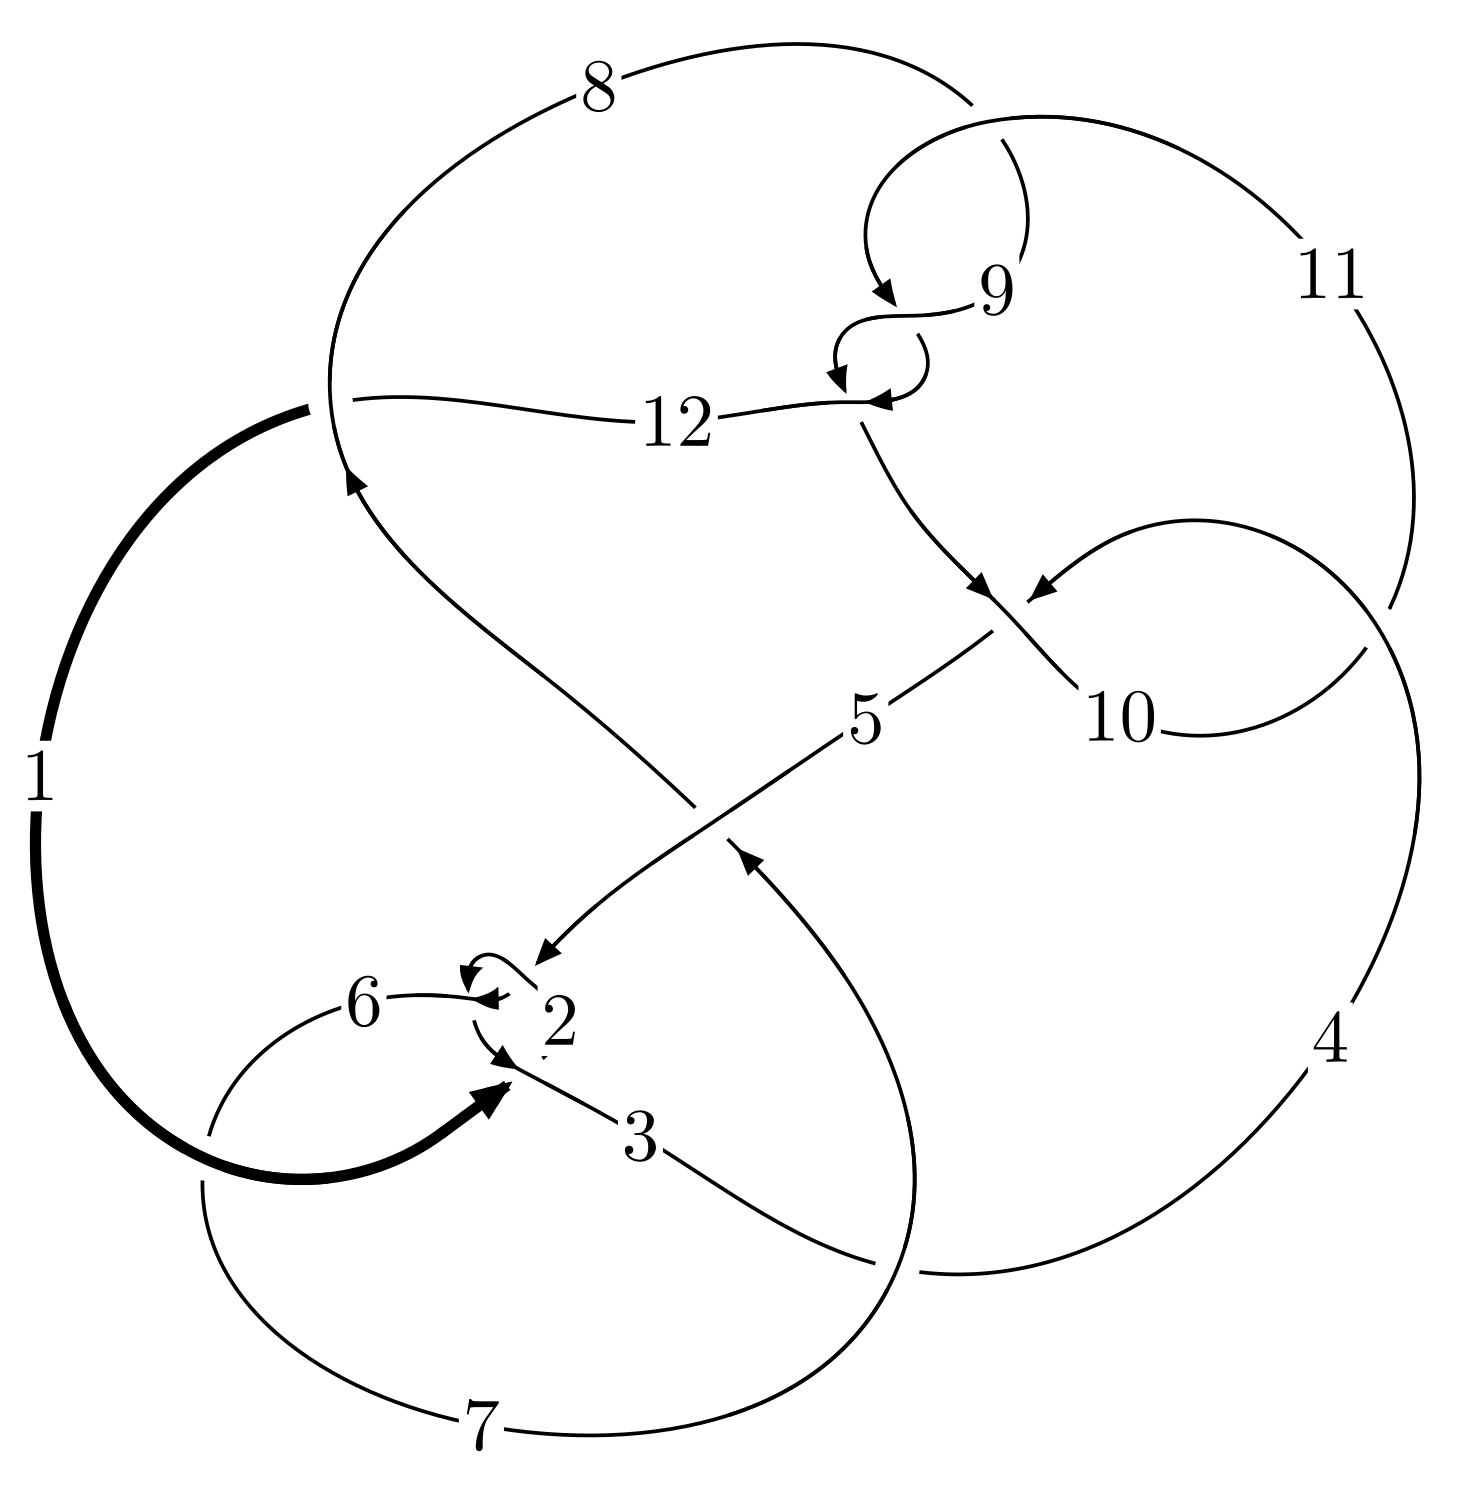
\includegraphics[width=112pt]{../../../GIT/diagram.site/Diagrams/png/1043_12a_0242.png}\\
\ \ \ A knot diagram\footnotemark}&
\allowdisplaybreaks
\textbf{Linearized knot diagam} \\
\cline{2-2}
 &
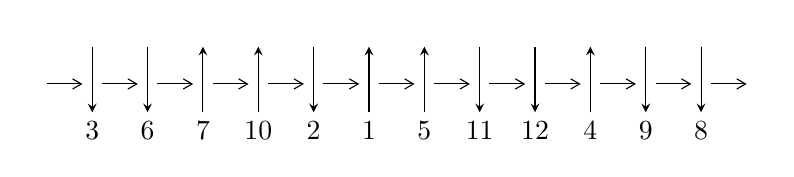
\begin{tikzpicture}[x=20pt, y=17pt]
	% nodes
	\node (C0) at (0, 0) {};
	\node (C1) at (1, 0) {};
	\node (C1U) at (1, +1) {};
	\node (C1D) at (1, -1) {3};

	\node (C2) at (2, 0) {};
	\node (C2U) at (2, +1) {};
	\node (C2D) at (2, -1) {6};

	\node (C3) at (3, 0) {};
	\node (C3U) at (3, +1) {};
	\node (C3D) at (3, -1) {7};

	\node (C4) at (4, 0) {};
	\node (C4U) at (4, +1) {};
	\node (C4D) at (4, -1) {10};

	\node (C5) at (5, 0) {};
	\node (C5U) at (5, +1) {};
	\node (C5D) at (5, -1) {2};

	\node (C6) at (6, 0) {};
	\node (C6U) at (6, +1) {};
	\node (C6D) at (6, -1) {1};

	\node (C7) at (7, 0) {};
	\node (C7U) at (7, +1) {};
	\node (C7D) at (7, -1) {5};

	\node (C8) at (8, 0) {};
	\node (C8U) at (8, +1) {};
	\node (C8D) at (8, -1) {11};

	\node (C9) at (9, 0) {};
	\node (C9U) at (9, +1) {};
	\node (C9D) at (9, -1) {12};

	\node (C10) at (10, 0) {};
	\node (C10U) at (10, +1) {};
	\node (C10D) at (10, -1) {4};

	\node (C11) at (11, 0) {};
	\node (C11U) at (11, +1) {};
	\node (C11D) at (11, -1) {9};

	\node (C12) at (12, 0) {};
	\node (C12U) at (12, +1) {};
	\node (C12D) at (12, -1) {8};
	\node (C13) at (13, 0) {};

	% arrows
	\draw[->,>={angle 60}]
	(C0) edge (C1) (C1) edge (C2) (C2) edge (C3) (C3) edge (C4) (C4) edge (C5) (C5) edge (C6) (C6) edge (C7) (C7) edge (C8) (C8) edge (C9) (C9) edge (C10) (C10) edge (C11) (C11) edge (C12) (C12) edge (C13) ;	\draw[->,>=stealth]
	(C1U) edge (C1D) (C2U) edge (C2D) (C3D) edge (C3U) (C4D) edge (C4U) (C5U) edge (C5D) (C6D) edge (C6U) (C7D) edge (C7U) (C8U) edge (C8D) (C9U) edge (C9D) (C10D) edge (C10U) (C11U) edge (C11D) (C12U) edge (C12D) ;
	\end{tikzpicture} \\
\hhline{~~} \\& 
\textbf{Solving Sequence} \\ \cline{2-2} 
 &
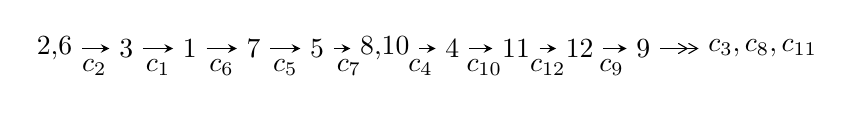
\begin{tikzpicture}[x=23pt, y=7pt]
	% node
	\node (A0) at (-1/8, 0) {2,6};
	\node (A1) at (1, 0) {3};
	\node (A2) at (2, 0) {1};
	\node (A3) at (3, 0) {7};
	\node (A4) at (4, 0) {5};
	\node (A5) at (81/16, 0) {8,10};
	\node (A6) at (49/8, 0) {4};
	\node (A7) at (57/8, 0) {11};
	\node (A8) at (65/8, 0) {12};
	\node (A9) at (73/8, 0) {9};
	\node (C1) at (1/2, -1) {$c_{2}$};
	\node (C2) at (3/2, -1) {$c_{1}$};
	\node (C3) at (5/2, -1) {$c_{6}$};
	\node (C4) at (7/2, -1) {$c_{5}$};
	\node (C5) at (9/2, -1) {$c_{7}$};
	\node (C6) at (45/8, -1) {$c_{4}$};
	\node (C7) at (53/8, -1) {$c_{10}$};
	\node (C8) at (61/8, -1) {$c_{12}$};
	\node (C9) at (69/8, -1) {$c_{9}$};
	\node (A10) at (11, 0) {$c_{3},c_{8},c_{11}$};

	% edge
	\draw[->,>=stealth]	
	(A0) edge (A1) (A1) edge (A2) (A2) edge (A3) (A3) edge (A4) (A4) edge (A5) (A5) edge (A6) (A6) edge (A7) (A7) edge (A8) (A8) edge (A9) ;
	\draw[->>,>={angle 60}]	
	(A9) edge (A10);
\end{tikzpicture} \\ 

\end{tabular} \\

\footnotetext{
The image of knot diagram is generated by the software ``\textbf{Draw programme}" developed by Andrew Bartholomew(\url{http://www.layer8.co.uk/maths/draw/index.htm\#Running-draw}), where we modified some parts for our purpose(\url{https://github.com/CATsTAILs/LinksPainter}).
}\phantom \\ \newline 
\centering \textbf{Ideals for irreducible components\footnotemark of $X_{\text{par}}$} 
 
\begin{align*}
I^u_{1}&=\langle 
- u^{100}+2 u^{99}+\cdots+b+1,\;u^{99}- u^{98}+\cdots+a+u,\;u^{101}-2 u^{100}+\cdots-3 u+1\rangle \\
I^u_{2}&=\langle 
- u^5- u^4+u^3+u^2+b,\;- u^5- u^4+u^3+u^2+a,\;u^6+u^5- u^4-2 u^3+u+1\rangle \\
\\
\end{align*}
\raggedright * 2 irreducible components of $\dim_{\mathbb{C}}=0$, with total 107 representations.\\
\footnotetext{All coefficients of polynomials are rational numbers. But the coefficients are sometimes approximated in decimal forms when there is not enough margin.}
\newpage
\renewcommand{\arraystretch}{1}
\centering \section*{I. $I^u_{1}= \langle - u^{100}+2 u^{99}+\cdots+b+1,\;u^{99}- u^{98}+\cdots+a+u,\;u^{101}-2 u^{100}+\cdots-3 u+1 \rangle$}
\flushleft \textbf{(i) Arc colorings}\\
\begin{tabular}{m{7pt} m{180pt} m{7pt} m{180pt} }
\flushright $a_{2}=$&$\begin{pmatrix}1\\0\end{pmatrix}$ \\
\flushright $a_{6}=$&$\begin{pmatrix}0\\u\end{pmatrix}$ \\
\flushright $a_{3}=$&$\begin{pmatrix}1\\u^2\end{pmatrix}$ \\
\flushright $a_{1}=$&$\begin{pmatrix}- u^2+1\\- u^4\end{pmatrix}$ \\
\flushright $a_{7}=$&$\begin{pmatrix}u^5-2 u^3+u\\u^7- u^5+u\end{pmatrix}$ \\
\flushright $a_{5}=$&$\begin{pmatrix}u\\u\end{pmatrix}$ \\
\flushright $a_{8}=$&$\begin{pmatrix}u^9-2 u^7+3 u^5-2 u^3+u\\u^9- u^7+u^5+u\end{pmatrix}$ \\
\flushright $a_{10}=$&$\begin{pmatrix}- u^{99}+u^{98}+\cdots+2 u^2- u\\u^{100}-2 u^{99}+\cdots+2 u-1\end{pmatrix}$ \\
\flushright $a_{4}=$&$\begin{pmatrix}- u^{10}+3 u^8-4 u^6+3 u^4- u^2+1\\- u^{12}+2 u^{10}-2 u^8+u^4\end{pmatrix}$ \\
\flushright $a_{11}=$&$\begin{pmatrix}- u^{99}+u^{98}+\cdots-4 u+1\\- u^{100}+25 u^{98}+\cdots-3 u+1\end{pmatrix}$ \\
\flushright $a_{12}=$&$\begin{pmatrix}- u^{22}+5 u^{20}+\cdots-2 u^2+1\\- u^{22}+4 u^{20}-9 u^{18}+12 u^{16}-12 u^{14}+10 u^{12}-9 u^{10}+6 u^8-3 u^6- u^2\end{pmatrix}$ \\
\flushright $a_{9}=$&$\begin{pmatrix}- u^{99}+u^{98}+\cdots-2 u+1\\- u^{99}+u^{98}+\cdots-2 u^3+2 u^2\end{pmatrix}$\\&\end{tabular}
\flushleft \textbf{(ii) Obstruction class $= -1$}\\~\\
\flushleft \textbf{(iii) Cusp Shapes $= 12 u^{100}-14 u^{99}+\cdots+24 u-14$}\\~\\
\newpage\renewcommand{\arraystretch}{1}
\flushleft \textbf{(iv) u-Polynomials at the component}\newline \\
\begin{tabular}{m{50pt}|m{274pt}}
Crossings & \hspace{64pt}u-Polynomials at each crossing \\
\hline $$\begin{aligned}c_{1}\end{aligned}$$&$\begin{aligned}
&u^{101}+48 u^{100}+\cdots+5 u+1
\end{aligned}$\\
\hline $$\begin{aligned}c_{2},c_{5}\end{aligned}$$&$\begin{aligned}
&u^{101}+2 u^{100}+\cdots-3 u-1
\end{aligned}$\\
\hline $$\begin{aligned}c_{3}\end{aligned}$$&$\begin{aligned}
&u^{101}-2 u^{100}+\cdots-20923 u-4753
\end{aligned}$\\
\hline $$\begin{aligned}c_{4},c_{10}\end{aligned}$$&$\begin{aligned}
&u^{101}+u^{100}+\cdots+192 u+64
\end{aligned}$\\
\hline $$\begin{aligned}c_{6}\end{aligned}$$&$\begin{aligned}
&u^{101}+6 u^{100}+\cdots-4249 u-935
\end{aligned}$\\
\hline $$\begin{aligned}c_{7}\end{aligned}$$&$\begin{aligned}
&u^{101}+12 u^{100}+\cdots+15457 u+841
\end{aligned}$\\
\hline $$\begin{aligned}c_{8},c_{9},c_{11}\end{aligned}$$&$\begin{aligned}
&u^{101}-7 u^{100}+\cdots-6 u+1
\end{aligned}$\\
\hline $$\begin{aligned}c_{12}\end{aligned}$$&$\begin{aligned}
&u^{101}+39 u^{100}+\cdots-24576 u-4096
\end{aligned}$\\
\hline
\end{tabular}\\~\\
\newpage\renewcommand{\arraystretch}{1}
\flushleft \textbf{(v) Riley Polynomials at the component}\newline \\
\begin{tabular}{m{50pt}|m{274pt}}
Crossings & \hspace{64pt}Riley Polynomials at each crossing \\
\hline $$\begin{aligned}c_{1}\end{aligned}$$&$\begin{aligned}
&y^{101}+12 y^{100}+\cdots-3 y-1
\end{aligned}$\\
\hline $$\begin{aligned}c_{2},c_{5}\end{aligned}$$&$\begin{aligned}
&y^{101}-48 y^{100}+\cdots+5 y-1
\end{aligned}$\\
\hline $$\begin{aligned}c_{3}\end{aligned}$$&$\begin{aligned}
&y^{101}-24 y^{100}+\cdots+1248690765 y-22591009
\end{aligned}$\\
\hline $$\begin{aligned}c_{4},c_{10}\end{aligned}$$&$\begin{aligned}
&y^{101}+39 y^{100}+\cdots-24576 y-4096
\end{aligned}$\\
\hline $$\begin{aligned}c_{6}\end{aligned}$$&$\begin{aligned}
&y^{101}+24 y^{100}+\cdots-42754659 y-874225
\end{aligned}$\\
\hline $$\begin{aligned}c_{7}\end{aligned}$$&$\begin{aligned}
&y^{101}+12 y^{100}+\cdots+19680241 y-707281
\end{aligned}$\\
\hline $$\begin{aligned}c_{8},c_{9},c_{11}\end{aligned}$$&$\begin{aligned}
&y^{101}-87 y^{100}+\cdots+14 y-1
\end{aligned}$\\
\hline $$\begin{aligned}c_{12}\end{aligned}$$&$\begin{aligned}
&y^{101}+35 y^{100}+\cdots+452984832 y-16777216
\end{aligned}$\\
\hline
\end{tabular}\\~\\
\newpage\flushleft \textbf{(vi) Complex Volumes and Cusp Shapes}
$$\begin{array}{c|c|c}  
\text{Solutions to }I^u_{1}& \I (\text{vol} + \sqrt{-1}CS) & \text{Cusp shape}\\
 \hline 
\begin{aligned}
u &= \phantom{-}1.052420 + 0.128459 I \\
a &= \phantom{-}0.1398400 - 0.0153419 I \\
b &= \phantom{-}0.432857 - 0.949399 I\end{aligned}
 & -4.78922 - 2.77784 I & \phantom{-0.000000 } 0 \\ \hline\begin{aligned}
u &= \phantom{-}1.052420 - 0.128459 I \\
a &= \phantom{-}0.1398400 + 0.0153419 I \\
b &= \phantom{-}0.432857 + 0.949399 I\end{aligned}
 & -4.78922 + 2.77784 I & \phantom{-0.000000 } 0 \\ \hline\begin{aligned}
u &= \phantom{-}0.755068 + 0.557624 I \\
a &= \phantom{-}0.102973 + 0.282474 I \\
b &= -0.578772 - 0.739571 I\end{aligned}
 & -6.39865 - 2.23005 I & \phantom{-0.000000 } 0 \\ \hline\begin{aligned}
u &= \phantom{-}0.755068 - 0.557624 I \\
a &= \phantom{-}0.102973 - 0.282474 I \\
b &= -0.578772 + 0.739571 I\end{aligned}
 & -6.39865 + 2.23005 I & \phantom{-0.000000 } 0 \\ \hline\begin{aligned}
u &= \phantom{-}0.633815 + 0.669876 I \\
a &= \phantom{-}0.580927 + 0.080737 I \\
b &= \phantom{-}0.92685 + 1.45655 I\end{aligned}
 & -1.26580 - 9.60369 I & \phantom{-0.000000 } 0 \\ \hline\begin{aligned}
u &= \phantom{-}0.633815 - 0.669876 I \\
a &= \phantom{-}0.580927 - 0.080737 I \\
b &= \phantom{-}0.92685 - 1.45655 I\end{aligned}
 & -1.26580 + 9.60369 I & \phantom{-0.000000 } 0 \\ \hline\begin{aligned}
u &= \phantom{-}1.030840 + 0.337224 I \\
a &= -0.046217 + 0.243872 I \\
b &= \phantom{-}0.457897 + 0.352581 I\end{aligned}
 & -1.96756 - 1.35415 I & \phantom{-0.000000 } 0 \\ \hline\begin{aligned}
u &= \phantom{-}1.030840 - 0.337224 I \\
a &= -0.046217 - 0.243872 I \\
b &= \phantom{-}0.457897 - 0.352581 I\end{aligned}
 & -1.96756 + 1.35415 I & \phantom{-0.000000 } 0 \\ \hline\begin{aligned}
u &= \phantom{-}1.070010 + 0.217154 I \\
a &= -0.199686 - 0.063001 I \\
b &= -0.705802 + 0.573504 I\end{aligned}
 & -0.934930 - 0.044176 I & \phantom{-0.000000 } 0 \\ \hline\begin{aligned}
u &= \phantom{-}1.070010 - 0.217154 I \\
a &= -0.199686 + 0.063001 I \\
b &= -0.705802 - 0.573504 I\end{aligned}
 & -0.934930 + 0.044176 I & \phantom{-0.000000 } 0\\
 \hline 
 \end{array}$$\newpage$$\begin{array}{c|c|c}  
\text{Solutions to }I^u_{1}& \I (\text{vol} + \sqrt{-1}CS) & \text{Cusp shape}\\
 \hline 
\begin{aligned}
u &= \phantom{-}0.609804 + 0.654819 I \\
a &= -0.509436 - 0.264760 I \\
b &= -0.79698 - 1.54382 I\end{aligned}
 & \phantom{-}3.60239 - 5.43636 I & \phantom{-0.000000 -}0. + 6.67139 I \\ \hline\begin{aligned}
u &= \phantom{-}0.609804 - 0.654819 I \\
a &= -0.509436 + 0.264760 I \\
b &= -0.79698 + 1.54382 I\end{aligned}
 & \phantom{-}3.60239 + 5.43636 I & \phantom{-0.000000 } 0. - 6.67139 I \\ \hline\begin{aligned}
u &= \phantom{-}0.938435 + 0.588259 I \\
a &= -0.842077 - 0.734205 I \\
b &= \phantom{-}0.197316 - 0.238136 I\end{aligned}
 & -2.16486 + 4.72332 I & \phantom{-0.000000 } 0 \\ \hline\begin{aligned}
u &= \phantom{-}0.938435 - 0.588259 I \\
a &= -0.842077 + 0.734205 I \\
b &= \phantom{-}0.197316 + 0.238136 I\end{aligned}
 & -2.16486 - 4.72332 I & \phantom{-0.000000 } 0 \\ \hline\begin{aligned}
u &= -0.966470 + 0.548870 I \\
a &= \phantom{-}1.28398 - 0.83171 I \\
b &= \phantom{-}0.88047 - 1.68436 I\end{aligned}
 & -0.672587 + 1.029480 I & \phantom{-0.000000 } 0 \\ \hline\begin{aligned}
u &= -0.966470 - 0.548870 I \\
a &= \phantom{-}1.28398 + 0.83171 I \\
b &= \phantom{-}0.88047 + 1.68436 I\end{aligned}
 & -0.672587 - 1.029480 I & \phantom{-0.000000 } 0 \\ \hline\begin{aligned}
u &= \phantom{-}0.959435 + 0.569390 I \\
a &= \phantom{-}1.041610 + 0.586251 I \\
b &= \phantom{-}0.099199 + 0.178007 I\end{aligned}
 & \phantom{-}2.57284 + 0.65864 I & \phantom{-0.000000 } 0 \\ \hline\begin{aligned}
u &= \phantom{-}0.959435 - 0.569390 I \\
a &= \phantom{-}1.041610 - 0.586251 I \\
b &= \phantom{-}0.099199 - 0.178007 I\end{aligned}
 & \phantom{-}2.57284 - 0.65864 I & \phantom{-0.000000 } 0 \\ \hline\begin{aligned}
u &= -0.534368 + 0.701148 I \\
a &= -0.818876 + 0.909716 I \\
b &= \phantom{-}0.359753 + 0.781522 I\end{aligned}
 & \phantom{-}0.58025 - 3.29880 I & \phantom{-0.000000 -}0. + 3.45551 I \\ \hline\begin{aligned}
u &= -0.534368 - 0.701148 I \\
a &= -0.818876 - 0.909716 I \\
b &= \phantom{-}0.359753 - 0.781522 I\end{aligned}
 & \phantom{-}0.58025 + 3.29880 I & \phantom{-0.000000 } 0. - 3.45551 I\\
 \hline 
 \end{array}$$\newpage$$\begin{array}{c|c|c}  
\text{Solutions to }I^u_{1}& \I (\text{vol} + \sqrt{-1}CS) & \text{Cusp shape}\\
 \hline 
\begin{aligned}
u &= -0.602981 + 0.633411 I \\
a &= -1.23643 + 0.76240 I \\
b &= -0.033260 + 1.072500 I\end{aligned}
 & \phantom{-}0.39493 + 3.62199 I & \phantom{-0.000000 } 0. - 4.25248 I \\ \hline\begin{aligned}
u &= -0.602981 - 0.633411 I \\
a &= -1.23643 - 0.76240 I \\
b &= -0.033260 - 1.072500 I\end{aligned}
 & \phantom{-}0.39493 - 3.62199 I & \phantom{-0.000000 -}0. + 4.25248 I \\ \hline\begin{aligned}
u &= -1.098480 + 0.249907 I \\
a &= \phantom{-}1.46633 + 2.09687 I \\
b &= \phantom{-}0.95181 + 2.80503 I\end{aligned}
 & -4.54068 - 0.41043 I & \phantom{-0.000000 } 0 \\ \hline\begin{aligned}
u &= -1.098480 - 0.249907 I \\
a &= \phantom{-}1.46633 - 2.09687 I \\
b &= \phantom{-}0.95181 - 2.80503 I\end{aligned}
 & -4.54068 + 0.41043 I & \phantom{-0.000000 } 0 \\ \hline\begin{aligned}
u &= \phantom{-}0.991961 + 0.547840 I \\
a &= -1.371260 - 0.274593 I \\
b &= -0.568754 + 0.042247 I\end{aligned}
 & -0.36209 - 3.54745 I & \phantom{-0.000000 } 0 \\ \hline\begin{aligned}
u &= \phantom{-}0.991961 - 0.547840 I \\
a &= -1.371260 + 0.274593 I \\
b &= -0.568754 - 0.042247 I\end{aligned}
 & -0.36209 + 3.54745 I & \phantom{-0.000000 } 0 \\ \hline\begin{aligned}
u &= -0.559631 + 0.661068 I \\
a &= \phantom{-}1.023780 - 0.774703 I \\
b &= -0.135780 - 0.895963 I\end{aligned}
 & \phantom{-}4.42732 + 0.11667 I & \phantom{-}4.83665 + 0. I\phantom{ +0.000000I} \\ \hline\begin{aligned}
u &= -0.559631 - 0.661068 I \\
a &= \phantom{-}1.023780 + 0.774703 I \\
b &= -0.135780 + 0.895963 I\end{aligned}
 & \phantom{-}4.42732 - 0.11667 I & \phantom{-}4.83665 + 0. I\phantom{ +0.000000I} \\ \hline\begin{aligned}
u &= \phantom{-}1.114920 + 0.238092 I \\
a &= \phantom{-}0.284121 + 0.095472 I \\
b &= \phantom{-}1.059400 - 0.516964 I\end{aligned}
 & -5.34739 + 2.98728 I & \phantom{-0.000000 } 0 \\ \hline\begin{aligned}
u &= \phantom{-}1.114920 - 0.238092 I \\
a &= \phantom{-}0.284121 - 0.095472 I \\
b &= \phantom{-}1.059400 + 0.516964 I\end{aligned}
 & -5.34739 - 2.98728 I & \phantom{-0.000000 } 0\\
 \hline 
 \end{array}$$\newpage$$\begin{array}{c|c|c}  
\text{Solutions to }I^u_{1}& \I (\text{vol} + \sqrt{-1}CS) & \text{Cusp shape}\\
 \hline 
\begin{aligned}
u &= -1.120580 + 0.224260 I \\
a &= -1.34807 - 1.71177 I \\
b &= -0.64781 - 2.48601 I\end{aligned}
 & -2.28390 - 4.97717 I & \phantom{-0.000000 } 0 \\ \hline\begin{aligned}
u &= -1.120580 - 0.224260 I \\
a &= -1.34807 + 1.71177 I \\
b &= -0.64781 + 2.48601 I\end{aligned}
 & -2.28390 + 4.97717 I & \phantom{-0.000000 } 0 \\ \hline\begin{aligned}
u &= -1.097540 + 0.321538 I \\
a &= \phantom{-}0.62090 + 2.60978 I \\
b &= \phantom{-}0.52128 + 3.42738 I\end{aligned}
 & -5.22703 + 0.81000 I & \phantom{-0.000000 } 0 \\ \hline\begin{aligned}
u &= -1.097540 - 0.321538 I \\
a &= \phantom{-}0.62090 - 2.60978 I \\
b &= \phantom{-}0.52128 - 3.42738 I\end{aligned}
 & -5.22703 - 0.81000 I & \phantom{-0.000000 } 0 \\ \hline\begin{aligned}
u &= -0.418601 + 0.745337 I \\
a &= -0.031445 - 1.080460 I \\
b &= -0.636462 - 0.121876 I\end{aligned}
 & -0.004549 + 0.828463 I & -2.59773 - 3.39866 I \\ \hline\begin{aligned}
u &= -0.418601 - 0.745337 I \\
a &= -0.031445 + 1.080460 I \\
b &= -0.636462 + 0.121876 I\end{aligned}
 & -0.004549 - 0.828463 I & -2.59773 + 3.39866 I \\ \hline\begin{aligned}
u &= \phantom{-}0.341589 + 0.777836 I \\
a &= \phantom{-}2.60469 + 0.69821 I \\
b &= \phantom{-}1.029160 + 0.935138 I\end{aligned}
 & -2.75864 + 11.91880 I & -3.31016 - 7.20088 I \\ \hline\begin{aligned}
u &= \phantom{-}0.341589 - 0.777836 I \\
a &= \phantom{-}2.60469 - 0.69821 I \\
b &= \phantom{-}1.029160 - 0.935138 I\end{aligned}
 & -2.75864 - 11.91880 I & -3.31016 + 7.20088 I \\ \hline\begin{aligned}
u &= -0.998781 + 0.571100 I \\
a &= -1.160180 + 0.609320 I \\
b &= -0.93422 + 1.48602 I\end{aligned}
 & \phantom{-}3.13296 + 4.68056 I & \phantom{-0.000000 } 0 \\ \hline\begin{aligned}
u &= -0.998781 - 0.571100 I \\
a &= -1.160180 - 0.609320 I \\
b &= -0.93422 - 1.48602 I\end{aligned}
 & \phantom{-}3.13296 - 4.68056 I & \phantom{-0.000000 } 0\\
 \hline 
 \end{array}$$\newpage$$\begin{array}{c|c|c}  
\text{Solutions to }I^u_{1}& \I (\text{vol} + \sqrt{-1}CS) & \text{Cusp shape}\\
 \hline 
\begin{aligned}
u &= \phantom{-}0.572328 + 0.624706 I \\
a &= \phantom{-}0.273818 + 0.545396 I \\
b &= \phantom{-}0.53365 + 1.66046 I\end{aligned}
 & \phantom{-}0.876218 - 1.073990 I & -0.47148 + 3.54648 I \\ \hline\begin{aligned}
u &= \phantom{-}0.572328 - 0.624706 I \\
a &= \phantom{-}0.273818 - 0.545396 I \\
b &= \phantom{-}0.53365 - 1.66046 I\end{aligned}
 & \phantom{-}0.876218 + 1.073990 I & -0.47148 - 3.54648 I \\ \hline\begin{aligned}
u &= \phantom{-}1.108560 + 0.343316 I \\
a &= -0.216053 - 0.426382 I \\
b &= -1.119240 - 0.438738 I\end{aligned}
 & -6.42822 - 3.14881 I & \phantom{-0.000000 } 0 \\ \hline\begin{aligned}
u &= \phantom{-}1.108560 - 0.343316 I \\
a &= -0.216053 + 0.426382 I \\
b &= -1.119240 + 0.438738 I\end{aligned}
 & -6.42822 + 3.14881 I & \phantom{-0.000000 } 0 \\ \hline\begin{aligned}
u &= -1.140370 + 0.219226 I \\
a &= \phantom{-}1.18416 + 1.60649 I \\
b &= \phantom{-}0.40484 + 2.47427 I\end{aligned}
 & -7.44620 - 9.17178 I & \phantom{-0.000000 } 0 \\ \hline\begin{aligned}
u &= -1.140370 - 0.219226 I \\
a &= \phantom{-}1.18416 - 1.60649 I \\
b &= \phantom{-}0.40484 - 2.47427 I\end{aligned}
 & -7.44620 + 9.17178 I & \phantom{-0.000000 } 0 \\ \hline\begin{aligned}
u &= \phantom{-}0.347158 + 0.760698 I \\
a &= -2.62218 - 0.68502 I \\
b &= -1.18577 - 0.88400 I\end{aligned}
 & \phantom{-}2.29536 + 7.62101 I & \phantom{-}0.67662 - 6.29564 I \\ \hline\begin{aligned}
u &= \phantom{-}0.347158 - 0.760698 I \\
a &= -2.62218 + 0.68502 I \\
b &= -1.18577 + 0.88400 I\end{aligned}
 & \phantom{-}2.29536 - 7.62101 I & \phantom{-}0.67662 + 6.29564 I \\ \hline\begin{aligned}
u &= -1.111800 + 0.363448 I \\
a &= -0.24482 - 2.31312 I \\
b &= -0.36784 - 3.24484 I\end{aligned}
 & -3.73764 + 5.11320 I & \phantom{-0.000000 } 0 \\ \hline\begin{aligned}
u &= -1.111800 - 0.363448 I \\
a &= -0.24482 + 2.31312 I \\
b &= -0.36784 + 3.24484 I\end{aligned}
 & -3.73764 - 5.11320 I & \phantom{-0.000000 } 0\\
 \hline 
 \end{array}$$\newpage$$\begin{array}{c|c|c}  
\text{Solutions to }I^u_{1}& \I (\text{vol} + \sqrt{-1}CS) & \text{Cusp shape}\\
 \hline 
\begin{aligned}
u &= -0.374481 + 0.736699 I \\
a &= \phantom{-}0.356343 + 1.067530 I \\
b &= \phantom{-}0.611684 - 0.079445 I\end{aligned}
 & \phantom{-}3.53001 - 2.28299 I & \phantom{-}3.74749 + 1.05855 I \\ \hline\begin{aligned}
u &= -0.374481 - 0.736699 I \\
a &= \phantom{-}0.356343 - 1.067530 I \\
b &= \phantom{-}0.611684 + 0.079445 I\end{aligned}
 & \phantom{-}3.53001 + 2.28299 I & \phantom{-}3.74749 - 1.05855 I \\ \hline\begin{aligned}
u &= -0.340956 + 0.748894 I \\
a &= -0.547438 - 1.193920 I \\
b &= -0.653813 + 0.195404 I\end{aligned}
 & -0.87772 - 5.64328 I & -2.11529 + 3.95512 I \\ \hline\begin{aligned}
u &= -0.340956 - 0.748894 I \\
a &= -0.547438 + 1.193920 I \\
b &= -0.653813 - 0.195404 I\end{aligned}
 & -0.87772 + 5.64328 I & -2.11529 - 3.95512 I \\ \hline\begin{aligned}
u &= -1.019800 + 0.591476 I \\
a &= \phantom{-}1.148060 - 0.373840 I \\
b &= \phantom{-}1.11297 - 1.29175 I\end{aligned}
 & -0.85273 + 8.26854 I & \phantom{-0.000000 } 0 \\ \hline\begin{aligned}
u &= -1.019800 - 0.591476 I \\
a &= \phantom{-}1.148060 + 0.373840 I \\
b &= \phantom{-}1.11297 + 1.29175 I\end{aligned}
 & -0.85273 - 8.26854 I & \phantom{-0.000000 } 0 \\ \hline\begin{aligned}
u &= -1.143830 + 0.294047 I \\
a &= -0.78969 - 2.09405 I \\
b &= -0.45626 - 3.15545 I\end{aligned}
 & -12.66950 - 0.31771 I & \phantom{-0.000000 } 0 \\ \hline\begin{aligned}
u &= -1.143830 - 0.294047 I \\
a &= -0.78969 + 2.09405 I \\
b &= -0.45626 + 3.15545 I\end{aligned}
 & -12.66950 + 0.31771 I & \phantom{-0.000000 } 0 \\ \hline\begin{aligned}
u &= \phantom{-}0.345911 + 0.731475 I \\
a &= \phantom{-}2.66528 + 0.61476 I \\
b &= \phantom{-}1.40337 + 0.66992 I\end{aligned}
 & -0.20007 + 2.98834 I & -2.71240 - 3.17778 I \\ \hline\begin{aligned}
u &= \phantom{-}0.345911 - 0.731475 I \\
a &= \phantom{-}2.66528 - 0.61476 I \\
b &= \phantom{-}1.40337 - 0.66992 I\end{aligned}
 & -0.20007 - 2.98834 I & -2.71240 + 3.17778 I\\
 \hline 
 \end{array}$$\newpage$$\begin{array}{c|c|c}  
\text{Solutions to }I^u_{1}& \I (\text{vol} + \sqrt{-1}CS) & \text{Cusp shape}\\
 \hline 
\begin{aligned}
u &= -1.139320 + 0.371305 I \\
a &= \phantom{-}0.31637 + 2.12611 I \\
b &= \phantom{-}0.48661 + 3.21867 I\end{aligned}
 & -9.15955 + 8.82637 I & \phantom{-0.000000 } 0 \\ \hline\begin{aligned}
u &= -1.139320 - 0.371305 I \\
a &= \phantom{-}0.31637 - 2.12611 I \\
b &= \phantom{-}0.48661 - 3.21867 I\end{aligned}
 & -9.15955 - 8.82637 I & \phantom{-0.000000 } 0 \\ \hline\begin{aligned}
u &= -1.077030 + 0.542858 I \\
a &= \phantom{-}0.071890 - 0.629892 I \\
b &= -0.283599 - 0.913705 I\end{aligned}
 & -0.45669 + 5.39599 I & \phantom{-0.000000 } 0 \\ \hline\begin{aligned}
u &= -1.077030 - 0.542858 I \\
a &= \phantom{-}0.071890 + 0.629892 I \\
b &= -0.283599 + 0.913705 I\end{aligned}
 & -0.45669 - 5.39599 I & \phantom{-0.000000 } 0 \\ \hline\begin{aligned}
u &= \phantom{-}1.100270 + 0.494755 I \\
a &= -0.32807 + 1.65232 I \\
b &= \phantom{-}0.27526 + 2.25742 I\end{aligned}
 & -2.87000 - 2.35849 I & \phantom{-0.000000 } 0 \\ \hline\begin{aligned}
u &= \phantom{-}1.100270 - 0.494755 I \\
a &= -0.32807 - 1.65232 I \\
b &= \phantom{-}0.27526 - 2.25742 I\end{aligned}
 & -2.87000 + 2.35849 I & \phantom{-0.000000 } 0 \\ \hline\begin{aligned}
u &= \phantom{-}0.259363 + 0.735630 I \\
a &= -2.40428 - 0.68228 I \\
b &= -0.805941 - 0.276762 I\end{aligned}
 & -8.48867 + 3.43756 I & -7.95352 - 2.84384 I \\ \hline\begin{aligned}
u &= \phantom{-}0.259363 - 0.735630 I \\
a &= -2.40428 + 0.68228 I \\
b &= -0.805941 + 0.276762 I\end{aligned}
 & -8.48867 - 3.43756 I & -7.95352 + 2.84384 I \\ \hline\begin{aligned}
u &= -1.107400 + 0.512207 I \\
a &= \phantom{-}0.130066 + 1.191490 I \\
b &= \phantom{-}0.80513 + 1.69395 I\end{aligned}
 & -5.28761 + 4.34357 I & \phantom{-0.000000 } 0 \\ \hline\begin{aligned}
u &= -1.107400 - 0.512207 I \\
a &= \phantom{-}0.130066 - 1.191490 I \\
b &= \phantom{-}0.80513 - 1.69395 I\end{aligned}
 & -5.28761 - 4.34357 I & \phantom{-0.000000 } 0\\
 \hline 
 \end{array}$$\newpage$$\begin{array}{c|c|c}  
\text{Solutions to }I^u_{1}& \I (\text{vol} + \sqrt{-1}CS) & \text{Cusp shape}\\
 \hline 
\begin{aligned}
u &= \phantom{-}1.129590 + 0.478328 I \\
a &= -0.14991 - 1.46790 I \\
b &= -0.92464 - 2.18332 I\end{aligned}
 & -8.43973 + 0.95842 I & \phantom{-0.000000 } 0 \\ \hline\begin{aligned}
u &= \phantom{-}1.129590 - 0.478328 I \\
a &= -0.14991 + 1.46790 I \\
b &= -0.92464 + 2.18332 I\end{aligned}
 & -8.43973 - 0.95842 I & \phantom{-0.000000 } 0 \\ \hline\begin{aligned}
u &= \phantom{-}1.108120 + 0.527727 I \\
a &= \phantom{-}0.13959 - 2.44107 I \\
b &= -0.23659 - 3.14177 I\end{aligned}
 & -3.82038 - 6.62383 I & \phantom{-0.000000 } 0 \\ \hline\begin{aligned}
u &= \phantom{-}1.108120 - 0.527727 I \\
a &= \phantom{-}0.13959 + 2.44107 I \\
b &= -0.23659 + 3.14177 I\end{aligned}
 & -3.82038 + 6.62383 I & \phantom{-0.000000 } 0 \\ \hline\begin{aligned}
u &= -1.090320 + 0.586037 I \\
a &= -0.794158 - 0.400622 I \\
b &= -1.41676 + 0.02390 I\end{aligned}
 & -1.98492 + 4.22859 I & \phantom{-0.000000 } 0 \\ \hline\begin{aligned}
u &= -1.090320 - 0.586037 I \\
a &= -0.794158 + 0.400622 I \\
b &= -1.41676 - 0.02390 I\end{aligned}
 & -1.98492 - 4.22859 I & \phantom{-0.000000 } 0 \\ \hline\begin{aligned}
u &= -1.106080 + 0.570992 I \\
a &= \phantom{-}0.642285 + 0.669252 I \\
b &= \phantom{-}1.40913 + 0.52941 I\end{aligned}
 & \phantom{-}1.38275 + 7.25833 I & \phantom{-0.000000 } 0 \\ \hline\begin{aligned}
u &= -1.106080 - 0.570992 I \\
a &= \phantom{-}0.642285 - 0.669252 I \\
b &= \phantom{-}1.40913 - 0.52941 I\end{aligned}
 & \phantom{-}1.38275 - 7.25833 I & \phantom{-0.000000 } 0 \\ \hline\begin{aligned}
u &= \phantom{-}1.114420 + 0.562555 I \\
a &= -0.81295 - 2.95978 I \\
b &= -0.81437 - 3.80458 I\end{aligned}
 & -2.44582 - 7.91446 I & \phantom{-0.000000 } 0 \\ \hline\begin{aligned}
u &= \phantom{-}1.114420 - 0.562555 I \\
a &= -0.81295 + 2.95978 I \\
b &= -0.81437 + 3.80458 I\end{aligned}
 & -2.44582 + 7.91446 I & \phantom{-0.000000 } 0\\
 \hline 
 \end{array}$$\newpage$$\begin{array}{c|c|c}  
\text{Solutions to }I^u_{1}& \I (\text{vol} + \sqrt{-1}CS) & \text{Cusp shape}\\
 \hline 
\begin{aligned}
u &= -0.407550 + 0.629321 I \\
a &= -0.677042 - 0.205606 I \\
b &= -0.244368 + 0.284778 I\end{aligned}
 & \phantom{-}1.49320 - 0.76735 I & \phantom{-}6.12300 + 0.96206 I \\ \hline\begin{aligned}
u &= -0.407550 - 0.629321 I \\
a &= -0.677042 + 0.205606 I \\
b &= -0.244368 - 0.284778 I\end{aligned}
 & \phantom{-}1.49320 + 0.76735 I & \phantom{-}6.12300 - 0.96206 I \\ \hline\begin{aligned}
u &= -1.120230 + 0.566440 I \\
a &= -0.667711 - 0.855882 I \\
b &= -1.59973 - 0.83078 I\end{aligned}
 & -3.16163 + 10.62420 I & \phantom{-0.000000 } 0 \\ \hline\begin{aligned}
u &= -1.120230 - 0.566440 I \\
a &= -0.667711 + 0.855882 I \\
b &= -1.59973 + 0.83078 I\end{aligned}
 & -3.16163 - 10.62420 I & \phantom{-0.000000 } 0 \\ \hline\begin{aligned}
u &= \phantom{-}1.135270 + 0.538064 I \\
a &= \phantom{-}0.52498 + 2.30671 I \\
b &= \phantom{-}0.87565 + 3.29608 I\end{aligned}
 & -11.02440 - 8.24194 I & \phantom{-0.000000 } 0 \\ \hline\begin{aligned}
u &= \phantom{-}1.135270 - 0.538064 I \\
a &= \phantom{-}0.52498 - 2.30671 I \\
b &= \phantom{-}0.87565 - 3.29608 I\end{aligned}
 & -11.02440 + 8.24194 I & \phantom{-0.000000 } 0 \\ \hline\begin{aligned}
u &= \phantom{-}1.121660 + 0.571763 I \\
a &= \phantom{-}1.02281 + 2.77205 I \\
b &= \phantom{-}0.93735 + 3.74422 I\end{aligned}
 & \phantom{-}0.01813 - 12.65240 I & \phantom{-0.000000 } 0 \\ \hline\begin{aligned}
u &= \phantom{-}1.121660 - 0.571763 I \\
a &= \phantom{-}1.02281 - 2.77205 I \\
b &= \phantom{-}0.93735 - 3.74422 I\end{aligned}
 & \phantom{-}0.01813 + 12.65240 I & \phantom{-0.000000 } 0 \\ \hline\begin{aligned}
u &= \phantom{-}1.128560 + 0.575455 I \\
a &= -1.06834 - 2.64436 I \\
b &= -0.96826 - 3.71918 I\end{aligned}
 & -5.0801 - 17.0054 I & \phantom{-0.000000 } 0 \\ \hline\begin{aligned}
u &= \phantom{-}1.128560 - 0.575455 I \\
a &= -1.06834 + 2.64436 I \\
b &= -0.96826 + 3.71918 I\end{aligned}
 & -5.0801 + 17.0054 I & \phantom{-0.000000 } 0\\
 \hline 
 \end{array}$$\newpage$$\begin{array}{c|c|c}  
\text{Solutions to }I^u_{1}& \I (\text{vol} + \sqrt{-1}CS) & \text{Cusp shape}\\
 \hline 
\begin{aligned}
u &= \phantom{-}0.283550 + 0.647515 I \\
a &= \phantom{-}2.23141 + 0.35424 I \\
b &= \phantom{-}1.074950 - 0.206995 I\end{aligned}
 & -1.48981 + 2.04466 I & -5.62916 - 3.79059 I \\ \hline\begin{aligned}
u &= \phantom{-}0.283550 - 0.647515 I \\
a &= \phantom{-}2.23141 - 0.35424 I \\
b &= \phantom{-}1.074950 + 0.206995 I\end{aligned}
 & -1.48981 - 2.04466 I & -5.62916 + 3.79059 I \\ \hline\begin{aligned}
u &= \phantom{-}0.112489 + 0.678879 I \\
a &= \phantom{-}1.98470 + 0.88755 I \\
b &= \phantom{-}0.480281 - 0.196783 I\end{aligned}
 & -5.59993 - 5.24861 I & -6.43481 + 3.80727 I \\ \hline\begin{aligned}
u &= \phantom{-}0.112489 - 0.678879 I \\
a &= \phantom{-}1.98470 - 0.88755 I \\
b &= \phantom{-}0.480281 + 0.196783 I\end{aligned}
 & -5.59993 + 5.24861 I & -6.43481 - 3.80727 I \\ \hline\begin{aligned}
u &= \phantom{-}0.555631 + 0.364904 I \\
a &= -0.478905 - 0.138519 I \\
b &= -0.050258 + 0.905826 I\end{aligned}
 & -0.57618 - 1.33093 I & -3.67880 + 6.04129 I \\ \hline\begin{aligned}
u &= \phantom{-}0.555631 - 0.364904 I \\
a &= -0.478905 + 0.138519 I \\
b &= -0.050258 - 0.905826 I\end{aligned}
 & -0.57618 + 1.33093 I & -3.67880 - 6.04129 I \\ \hline\begin{aligned}
u &= -0.223103 + 0.609649 I \\
a &= \phantom{-}1.28747 + 0.84230 I \\
b &= \phantom{-}0.462436 - 0.362061 I\end{aligned}
 & -2.87314 + 0.06313 I & -4.60896 + 0.44073 I \\ \hline\begin{aligned}
u &= -0.223103 - 0.609649 I \\
a &= \phantom{-}1.28747 - 0.84230 I \\
b &= \phantom{-}0.462436 + 0.362061 I\end{aligned}
 & -2.87314 - 0.06313 I & -4.60896 - 0.44073 I \\ \hline\begin{aligned}
u &= \phantom{-}0.134739 + 0.590370 I \\
a &= -1.83884 - 0.72913 I \\
b &= -0.565952 + 0.320273 I\end{aligned}
 & -0.36248 - 1.81610 I & -2.37443 + 3.66266 I \\ \hline\begin{aligned}
u &= \phantom{-}0.134739 - 0.590370 I \\
a &= -1.83884 + 0.72913 I \\
b &= -0.565952 - 0.320273 I\end{aligned}
 & -0.36248 + 1.81610 I & -2.37443 - 3.66266 I\\
 \hline 
 \end{array}$$\newpage$$\begin{array}{c|c|c}  
\text{Solutions to }I^u_{1}& \I (\text{vol} + \sqrt{-1}CS) & \text{Cusp shape}\\
 \hline 
\begin{aligned}
u &= -0.512467\phantom{ +0.000000I} \\
a &= \phantom{-}2.15131\phantom{ +0.000000I} \\
b &= \phantom{-}0.883872\phantom{ +0.000000I}\end{aligned}
 & -2.31617\phantom{ +0.000000I} & -2.44180\phantom{ +0.000000I}\\
 \hline 
 \end{array}$$\newpage\newpage\renewcommand{\arraystretch}{1}
\centering \section*{II. $I^u_{2}= \langle - u^5- u^4+u^3+u^2+b,\;- u^5- u^4+u^3+u^2+a,\;u^6+u^5- u^4-2 u^3+u+1 \rangle$}
\flushleft \textbf{(i) Arc colorings}\\
\begin{tabular}{m{7pt} m{180pt} m{7pt} m{180pt} }
\flushright $a_{2}=$&$\begin{pmatrix}1\\0\end{pmatrix}$ \\
\flushright $a_{6}=$&$\begin{pmatrix}0\\u\end{pmatrix}$ \\
\flushright $a_{3}=$&$\begin{pmatrix}1\\u^2\end{pmatrix}$ \\
\flushright $a_{1}=$&$\begin{pmatrix}- u^2+1\\- u^4\end{pmatrix}$ \\
\flushright $a_{7}=$&$\begin{pmatrix}u^5-2 u^3+u\\u^5+u^4-2 u^3- u^2+u+1\end{pmatrix}$ \\
\flushright $a_{5}=$&$\begin{pmatrix}u\\u\end{pmatrix}$ \\
\flushright $a_{8}=$&$\begin{pmatrix}u^2-1\\u^4\end{pmatrix}$ \\
\flushright $a_{10}=$&$\begin{pmatrix}u^5+u^4- u^3- u^2\\u^5+u^4- u^3- u^2\end{pmatrix}$ \\
\flushright $a_{4}=$&$\begin{pmatrix}u\\u\end{pmatrix}$ \\
\flushright $a_{11}=$&$\begin{pmatrix}u^5+u^4- u^3- u^2\\u^5+u^4- u^3- u^2\end{pmatrix}$ \\
\flushright $a_{12}=$&$\begin{pmatrix}- u^2+1\\- u^4\end{pmatrix}$ \\
\flushright $a_{9}=$&$\begin{pmatrix}u^5+u^4- u^3-1\\u^5+2 u^4- u^3- u^2\end{pmatrix}$\\&\end{tabular}
\flushleft \textbf{(ii) Obstruction class $= 1$}\\~\\
\flushleft \textbf{(iii) Cusp Shapes $= 4 u^4-3 u^2-3 u-3$}\\~\\
\newpage\renewcommand{\arraystretch}{1}
\flushleft \textbf{(iv) u-Polynomials at the component}\newline \\
\begin{tabular}{m{50pt}|m{274pt}}
Crossings & \hspace{64pt}u-Polynomials at each crossing \\
\hline $$\begin{aligned}c_{1},c_{6}\end{aligned}$$&$\begin{aligned}
&u^6-3 u^5+5 u^4-4 u^3+2 u^2- u+1
\end{aligned}$\\
\hline $$\begin{aligned}c_{2},c_{7}\end{aligned}$$&$\begin{aligned}
&u^6+u^5- u^4-2 u^3+u+1
\end{aligned}$\\
\hline $$\begin{aligned}c_{3},c_{5}\end{aligned}$$&$\begin{aligned}
&u^6- u^5- u^4+2 u^3- u+1
\end{aligned}$\\
\hline $$\begin{aligned}c_{4},c_{10},c_{12}\end{aligned}$$&$\begin{aligned}
&u^6
\end{aligned}$\\
\hline $$\begin{aligned}c_{8},c_{9}\end{aligned}$$&$\begin{aligned}
&(u-1)^6
\end{aligned}$\\
\hline $$\begin{aligned}c_{11}\end{aligned}$$&$\begin{aligned}
&(u+1)^6
\end{aligned}$\\
\hline
\end{tabular}\\~\\
\newpage\renewcommand{\arraystretch}{1}
\flushleft \textbf{(v) Riley Polynomials at the component}\newline \\
\begin{tabular}{m{50pt}|m{274pt}}
Crossings & \hspace{64pt}Riley Polynomials at each crossing \\
\hline $$\begin{aligned}c_{1},c_{6}\end{aligned}$$&$\begin{aligned}
&y^6+y^5+5 y^4+6 y^2+3 y+1
\end{aligned}$\\
\hline $$\begin{aligned}c_{2},c_{3},c_{5}\\c_{7}\end{aligned}$$&$\begin{aligned}
&y^6-3 y^5+5 y^4-4 y^3+2 y^2- y+1
\end{aligned}$\\
\hline $$\begin{aligned}c_{4},c_{10},c_{12}\end{aligned}$$&$\begin{aligned}
&y^6
\end{aligned}$\\
\hline $$\begin{aligned}c_{8},c_{9},c_{11}\end{aligned}$$&$\begin{aligned}
&(y-1)^6
\end{aligned}$\\
\hline
\end{tabular}\\~\\
\newpage\flushleft \textbf{(vi) Complex Volumes and Cusp Shapes}
$$\begin{array}{c|c|c}  
\text{Solutions to }I^u_{2}& \I (\text{vol} + \sqrt{-1}CS) & \text{Cusp shape}\\
 \hline 
\begin{aligned}
u &= \phantom{-}1.002190 + 0.295542 I \\
a &= -1.000940 + 0.863088 I \\
b &= -1.000940 + 0.863088 I\end{aligned}
 & -3.53554 - 0.92430 I & -6.79748 + 1.68215 I \\ \hline\begin{aligned}
u &= \phantom{-}1.002190 - 0.295542 I \\
a &= -1.000940 - 0.863088 I \\
b &= -1.000940 - 0.863088 I\end{aligned}
 & -3.53554 + 0.92430 I & -6.79748 - 1.68215 I \\ \hline\begin{aligned}
u &= -0.428243 + 0.664531 I \\
a &= -0.573013 + 0.494098 I \\
b &= -0.573013 + 0.494098 I\end{aligned}
 & \phantom{-}0.245672 - 0.924305 I & -1.96974 + 0.88960 I \\ \hline\begin{aligned}
u &= -0.428243 - 0.664531 I \\
a &= -0.573013 - 0.494098 I \\
b &= -0.573013 - 0.494098 I\end{aligned}
 & \phantom{-}0.245672 + 0.924305 I & -1.96974 - 0.88960 I \\ \hline\begin{aligned}
u &= -1.073950 + 0.558752 I \\
a &= \phantom{-}0.573950 - 0.818891 I \\
b &= \phantom{-}0.573950 - 0.818891 I\end{aligned}
 & -1.64493 + 5.69302 I & -5.23279 - 6.15196 I \\ \hline\begin{aligned}
u &= -1.073950 - 0.558752 I \\
a &= \phantom{-}0.573950 + 0.818891 I \\
b &= \phantom{-}0.573950 + 0.818891 I\end{aligned}
 & -1.64493 - 5.69302 I & -5.23279 + 6.15196 I\\
 \hline 
 \end{array}$$\newpage
\newpage\renewcommand{\arraystretch}{1}
\centering \section*{ III. u-Polynomials}
\begin{tabular}{m{50pt}|m{274pt}}
Crossings & \hspace{64pt}u-Polynomials at each crossing \\
\hline $$\begin{aligned}c_{1}\end{aligned}$$&$\begin{aligned}
&(u^6-3 u^5+5 u^4-4 u^3+2 u^2- u+1)(u^{101}+48 u^{100}+\cdots+5 u+1)
\end{aligned}$\\
\hline $$\begin{aligned}c_{2}\end{aligned}$$&$\begin{aligned}
&(u^6+u^5- u^4-2 u^3+u+1)(u^{101}+2 u^{100}+\cdots-3 u-1)
\end{aligned}$\\
\hline $$\begin{aligned}c_{3}\end{aligned}$$&$\begin{aligned}
&(u^6- u^5- u^4+2 u^3- u+1)(u^{101}-2 u^{100}+\cdots-20923 u-4753)
\end{aligned}$\\
\hline $$\begin{aligned}c_{4},c_{10}\end{aligned}$$&$\begin{aligned}
&u^6(u^{101}+u^{100}+\cdots+192 u+64)
\end{aligned}$\\
\hline $$\begin{aligned}c_{5}\end{aligned}$$&$\begin{aligned}
&(u^6- u^5- u^4+2 u^3- u+1)(u^{101}+2 u^{100}+\cdots-3 u-1)
\end{aligned}$\\
\hline $$\begin{aligned}c_{6}\end{aligned}$$&$\begin{aligned}
&(u^6-3 u^5+5 u^4-4 u^3+2 u^2- u+1)(u^{101}+6 u^{100}+\cdots-4249 u-935)
\end{aligned}$\\
\hline $$\begin{aligned}c_{7}\end{aligned}$$&$\begin{aligned}
&(u^6+u^5- u^4-2 u^3+u+1)(u^{101}+12 u^{100}+\cdots+15457 u+841)
\end{aligned}$\\
\hline $$\begin{aligned}c_{8},c_{9}\end{aligned}$$&$\begin{aligned}
&((u-1)^6)(u^{101}-7 u^{100}+\cdots-6 u+1)
\end{aligned}$\\
\hline $$\begin{aligned}c_{11}\end{aligned}$$&$\begin{aligned}
&((u+1)^6)(u^{101}-7 u^{100}+\cdots-6 u+1)
\end{aligned}$\\
\hline $$\begin{aligned}c_{12}\end{aligned}$$&$\begin{aligned}
&u^6(u^{101}+39 u^{100}+\cdots-24576 u-4096)
\end{aligned}$\\
\hline
\end{tabular}\newpage\renewcommand{\arraystretch}{1}
\centering \section*{ IV. Riley Polynomials}
\begin{tabular}{m{50pt}|m{274pt}}
Crossings & \hspace{64pt}Riley Polynomials at each crossing \\
\hline $$\begin{aligned}c_{1}\end{aligned}$$&$\begin{aligned}
&(y^6+y^5+5 y^4+6 y^2+3 y+1)(y^{101}+12 y^{100}+\cdots-3 y-1)
\end{aligned}$\\
\hline $$\begin{aligned}c_{2},c_{5}\end{aligned}$$&$\begin{aligned}
&(y^6-3 y^5+5 y^4-4 y^3+2 y^2- y+1)(y^{101}-48 y^{100}+\cdots+5 y-1)
\end{aligned}$\\
\hline $$\begin{aligned}c_{3}\end{aligned}$$&$\begin{aligned}
&(y^6-3 y^5+5 y^4-4 y^3+2 y^2- y+1)\\
&\cdot(y^{101}-24 y^{100}+\cdots+1248690765 y-22591009)
\end{aligned}$\\
\hline $$\begin{aligned}c_{4},c_{10}\end{aligned}$$&$\begin{aligned}
&y^6(y^{101}+39 y^{100}+\cdots-24576 y-4096)
\end{aligned}$\\
\hline $$\begin{aligned}c_{6}\end{aligned}$$&$\begin{aligned}
&(y^6+y^5+5 y^4+6 y^2+3 y+1)\\
&\cdot(y^{101}+24 y^{100}+\cdots-42754659 y-874225)
\end{aligned}$\\
\hline $$\begin{aligned}c_{7}\end{aligned}$$&$\begin{aligned}
&(y^6-3 y^5+5 y^4-4 y^3+2 y^2- y+1)\\
&\cdot(y^{101}+12 y^{100}+\cdots+19680241 y-707281)
\end{aligned}$\\
\hline $$\begin{aligned}c_{8},c_{9},c_{11}\end{aligned}$$&$\begin{aligned}
&((y-1)^6)(y^{101}-87 y^{100}+\cdots+14 y-1)
\end{aligned}$\\
\hline $$\begin{aligned}c_{12}\end{aligned}$$&$\begin{aligned}
&y^6(y^{101}+35 y^{100}+\cdots+4.52985\times10^{8} y-1.67772\times10^{7})
\end{aligned}$\\
\hline
\end{tabular}
\vskip 2pc
\end{document}